\documentclass[10pt]{article}
\usepackage{graphicx}
\usepackage[margin=1.5cm]{geometry}
\usepackage{amsmath}
\def\brcurs{{\mbox{$\resizebox{.16in}{.08in}{
\includegraphics{BoldR}}$}}}
\def\rcurs{{\mbox{$\resizebox{.16in}{.08in}{
\includegraphics{ScriptR}}$}}}

\begin{document}
\twocolumn

\title{Tuesday Warm-up: Electric Fields in Matter}
\author{Prof. Jordan C. Hanson}

\maketitle

\section{Memory Bank}

\small

\begin{itemize}
\item \textbf{Relative voltage}:
\begin{equation}
V = - \int_a^{b} \mathbf{E} \cdot d\mathbf{l}
\end{equation}
\item \textbf{The electric displacement}:
\begin{equation}
\mathbf{D} = \epsilon_0 \mathbf{E} + \mathbf{P}
\end{equation}
\item \textbf{Gauss' Law for electric displacement}:
\begin{equation}
\oint \mathbf{D} \cdot d\mathbf{a} = Q_{\rm f,enc}
\end{equation}
\item \textbf{Linear dielectric materials}:
\begin{align}
\mathbf{P} &= \epsilon_0\chi_{\rm e} \mathbf{E} \\
\mathbf{D} &= \epsilon_0 \left(1+\chi_{\rm e}\right)\mathbf{E} \\
\mathbf{D} &= \epsilon \mathbf{E} \\
\epsilon_{\rm r} &= \epsilon/\epsilon_0 = 1+\chi_{\rm e}
\end{align}
\end{itemize}

\begin{figure}
\centering
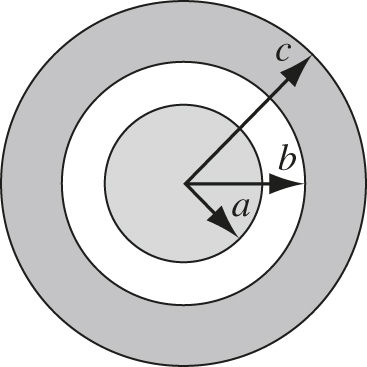
\includegraphics[width=0.2\textwidth]{figures/4_29.jpg}
\caption{\label{fig:1} A coaxial cable partially filled with a dielectric material with permittivity $\epsilon$.}
\end{figure}

\section{Linear Dielectric Materials}

\begin{enumerate}
\item Consider Fig. \ref{fig:1}.  A certain coaxial cable consists of a copper wire, radius $a$, surrounded by a concentric copper tube of inner radius $c$.  The space between is partially filled (from $b$ out to $c$) with material of diectric constant $\epsilon_{\rm r}$.  Find the capacitance per unit length of this cable.
\begin{itemize}
\item First, use Gauss' Law, with cylindrical symmetry, to find $\mathbf{D}$ for $a < s < c$. \\ \vspace{4cm}
\item Second, solve for $\mathbf{E}$, knowing that $\mathbf{D} = \epsilon \mathbf{E}$. \\ \vspace{2cm}
\item Third, obtain the voltage by integrating $\mathbf{E}$. \\ \vspace{4cm}
\item Fourth, use $Q = CV$ to solve for the capacitance, $C$.  What is $C$ in the limit $\epsilon_{\rm r} \to 1$? \\ \vspace{2cm}
\end{itemize}
\item Examine Tab. \ref{fig:2}.  The relationship between the \textit{dielectric constant} and the \textit{index of refraction} is $n \approx \sqrt{\epsilon_{\rm r}}$.  The speed of light is $c \approx 0.3$ m ns$^{-1}$.  Suppose a weather satellite radiates a microwave signal through 100 km of space, then 100 km of water vapor, and the signal reflects from the ocean and travels back to the satellite.  What is the time duration between transmission and reception?  What is the time for signals that travel through air?
\end{enumerate}

\begin{figure}[hb]
\centering
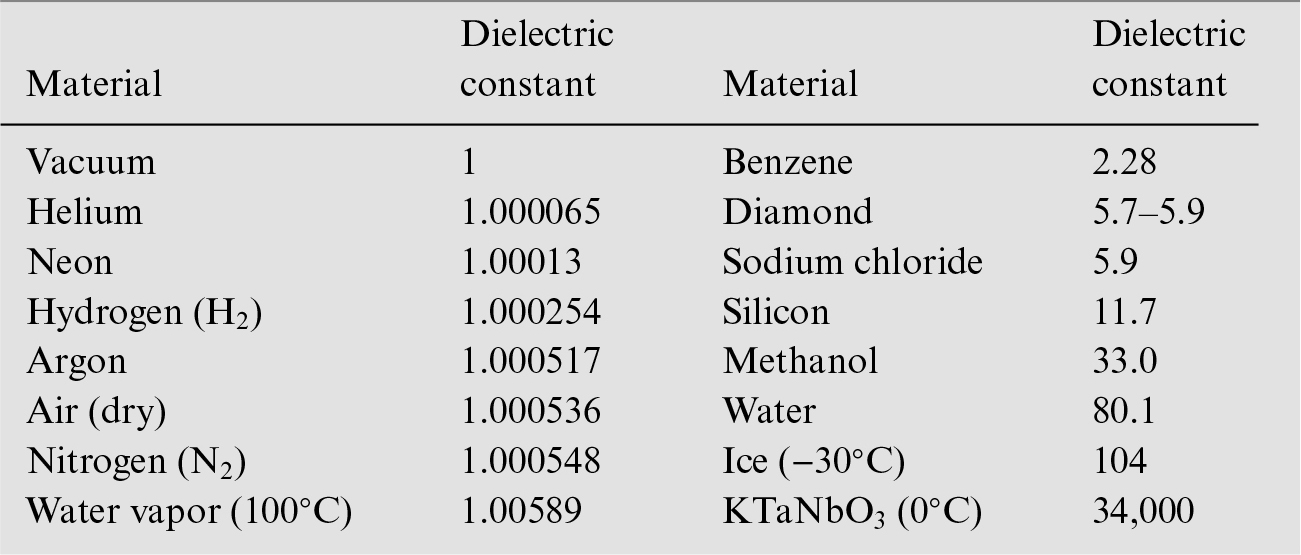
\includegraphics[width=0.45\textwidth]{figures/tab4_2.jpg}
\caption{\label{fig:2} Dielectric properties of different materials.}
\end{figure}

\end{document}
